\documentclass[../main.tex]{subfiles}

\begin{document}

\chapter{Drivers of Antarctic Ice}
\label{chap:environmenal_drivers}


% The variable which we found had the largest impact on the behaviour of ice in Antarctica is temperature. This follows naturally from the basic thermodynamics of phase change. As the temperature increases we see lower concentrations of sea ice, and as the temperature increases we see lower concentrations of sea ice. The extent of this relationship will be explored in detail in this chapter. We will first look at the relationship through density plots \textcolor{red}{Check name of plots}. Before calculating correlations and looking at the similarities and differences of the two different variables.

% For the purpose of this chapter, when we use temperature we will use \gls{skt} as discussed before \textcolor{red}{Write up different temperatures.}

% In chapter \ref{chap:temp_and_ice}, we found that temperature is significant for our understanding of the trends in Antarctic \gls{sic} over the last 40 years. However we found that the relationship between temperature and land ice is not as strong. To understand this we will have to do some more calculations.

% We want to consider a range of variables which could be impacting land ice in Antarctica. We will include temperature again for completeness. Wind speed is linked to atmospheric circulations which move clouds and thermal energy around the continent. Cloud cover has also been linked to behaviours in the land ice. \todo{add appropriate citations here}. 

Now we understand something of how ice in Antarctica has behaved over the last 40 years both over land and sea, we want to understand what dives the trends and variability which we have observed in chapter \ref{chap:ice_behaviour}. This will be the main focus of this chapter. First, we will briefly summarise the variables discussed in literature which we might expect to impact the behaviour of Antarctic ice. We will briefly revisit the technicalities of using the different datasets we have for different variables and the implications this has for our analysis. Then we will explore briefly some observational statistics for the different variables we are interested in. Plotting trends and mean timer-series for each variable and discussing any immediately apparent relationships between the different variables. We will carry out regression analysis, comparing each environmental variable with Antarctic ice, and finally we will do multi-regression analysis to complete our statistical analysis of what drives Antarctic Ice.

\section{Refresher on behaviour of Antarctic Ice}
Before continuing, we will include the figures from chapter \ref{chap:ice_behaviour} which show us how ice in Antarctica behaves. These figures are discussed in more detail where they are presented, however are included here for easy reference when comparing to the behaviour of other variables.
\missingfigure{Mean Ice Spatial}
\begin{figure}[hbt!]
    \centering
    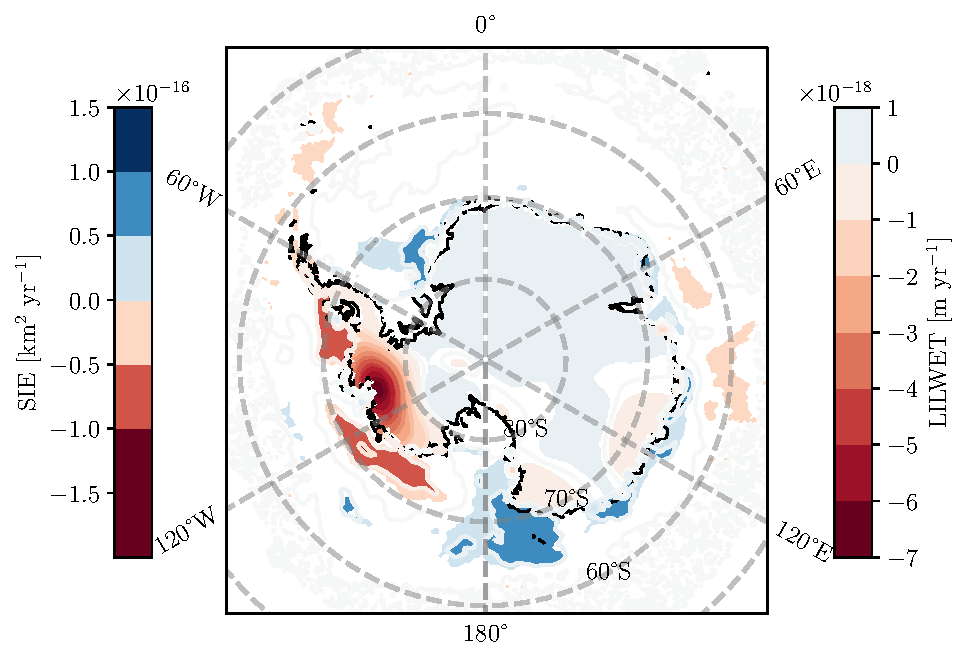
\includegraphics{images/T2/individually_made/hres/combined_ice_trend_0.05}
    \caption{Trends in Antarctic Land and Sea Ice.}
    \label{fig:combined_ice_trend_0}
\end{figure}
\missingfigure{Time-series of Antarctic Ice}

\section{Variables discussed in literature}
As we When people discuss behaviours in sea ice, they mostly discuss it in relationship to climate circulations such as \gls{enso} or \gls{sam}. While these circulations are important for our understanding of what drives the behaviour of ice in Antarctica if we consider only them, we miss the full story of what drives ice change in Antarctica. 

Instead we want to consider physical environmental variables such as temperature or surface pressure. For sea ice, environmental variables often linked to its behaviours are temperature of the atmosphere and ocean, solar radiation as its behaviour is tightly linked to the radiative balance, and temperature and salinity of the ocean. 

In regards to land ice, a number of theories have been put forward as to what drives the behaviours we see. Temperature, is again important, especially the temperature of the subsurface ocean. It is thought that increased ocean temperatures has lead to glaciers melting and flowing faster out to sea, this leading to a decrease in the mass of the glaciers and amount of land ice .Wind speed is linked to atmospheric circulations which move clouds and thermal energy around the continent. Cloud cover has also been linked to behaviours in the land ice. And finally we will consider ozone mass mixing ratios and total precipitation. It has been suggested that ozone concentrations can affect the precipitation above Antarctica, affecting the mass growth of the ice sheets.

\missingfigure{table of variables with their sources and time periods.}

Looking at the variables above we notice that not all of them are available on the same time-periods. Sea ice data and any data sourced from the ECMWF ERA5 reanalysis is available starting in 1979, however subsurface temperature data restricts us to 2002-2017, and land ice data restricts us to 2002-2019. In order to deal with this we will generally use the largest time period available for any given calculations. By default this will be 1979-2019, however anything involving land ice data will be restricted to 2002-2019. anything involving subsurface temperature will be further restricted to 2002-2017. Make sure to read the caption of any figure to ascertain what time periods were used.

\section{Trends in Variables}
Before doing any statistics, we want to look at the different variables from an observational standpoint. How are they behaving, and what does that mean for our understanding of how they might drive behaviours in Antarctic ice? We start this by plotting the spatial trends in each variable.

\missingfigure{Sub-figures of trends in each variable}

We start by looking at the spatial pattern of trends in \gls{skt} (see Figure \ref{fig:trend_skt_02_17}).
\begin{figure}[hbt!]
    \centering
    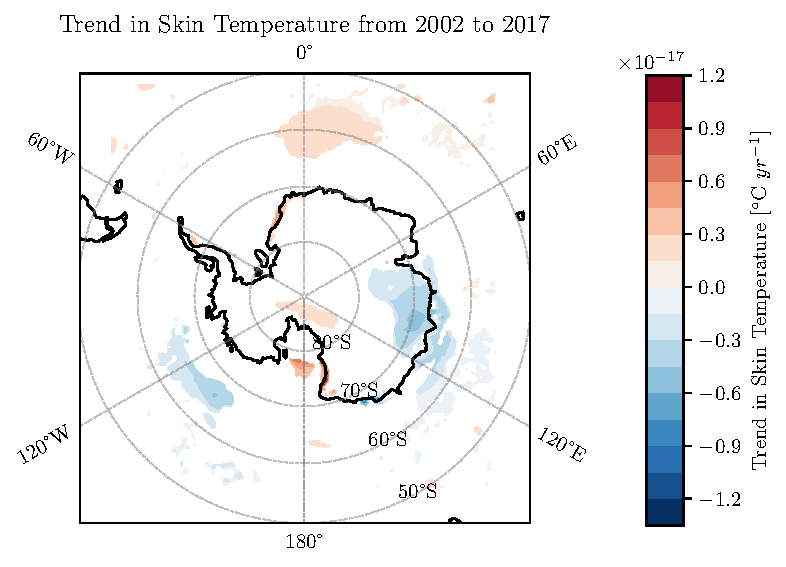
\includegraphics{images/2021w5/chapter7/hres/trend_spatial_skt}
    \caption{Trend in \gls{skt} over Antarctica from 2002 to 2017. Only statistically significant trends have been plotted, i.e. with a p-value $\leq$ 0.05.}
    \label{fig:trend_skt_02_17}
\end{figure}

Looking at the trend in \gls{skt} (figure \ref{fig:trend_skt_02_17}), we note that there is not a large region of the continent with statistically significant trends in \gls{skt} from 2002 to 2017. This is likely due to the large variability of temperature and the slowly moving trends. We can also look at the trends in subsurface oceanic temperatures (see Figure \ref{fig:trend_subsurtemp_02_17}) this is what has been predominantly proposed to have driven changes in Antarctic land ice by literature. The structure of the ocean and the temperature gradient is complicated and driven by a mixed layer close to the surface. To rigorously understand the relationship between land ice and oceanic temperatures, a condition for the depth of the mixed layer would have to be applied, \todo{add citation to paper from Melissa} however that is out of the scope of this thesis unless the results are exceptionally promising, which they are not. As a proxy for this we took the temperature at three different depths (100 dbar, 500 dbar, 700 dbar) and will be comparing these with the different ice variables. Our hope is that by considering a range of depths we will capture any physical processes occurring between land ice and subsurface temperatures without introducing more complicated considerations which would take more time to compute and introduce unnecessary errors in our results.
\begin{figure}[hbt!]
    \begin{subfigure}[b]{0.3\textwidth}
    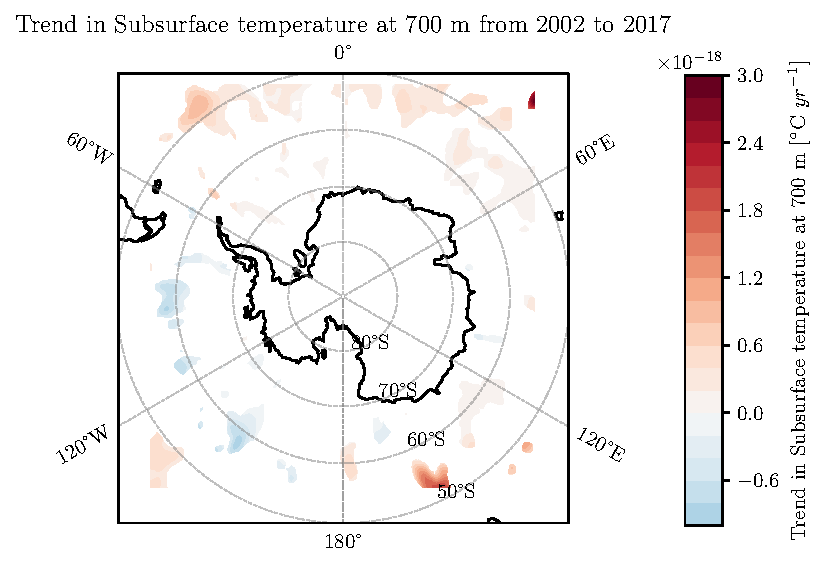
\includegraphics[width=\textwidth]{images/2021w5/chapter7/hres/trend_spatial_subsurtemp_700}
    \end{subfigure}
    \begin{subfigure}[b]{0.3\textwidth}
    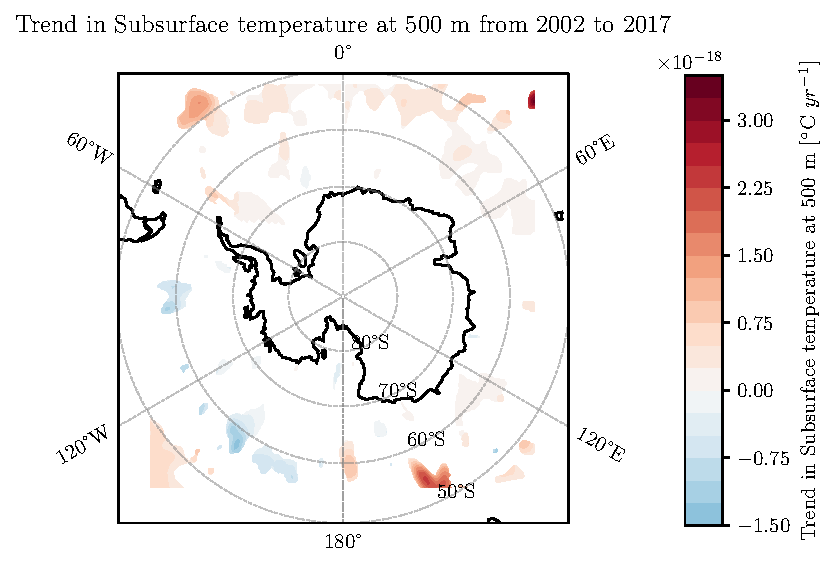
\includegraphics[width=\textwidth]{images/2021w5/chapter7/hres/trend_spatial_subsurtemp_500}
    \end{subfigure}
    \begin{subfigure}[b]{0.3\textwidth}
    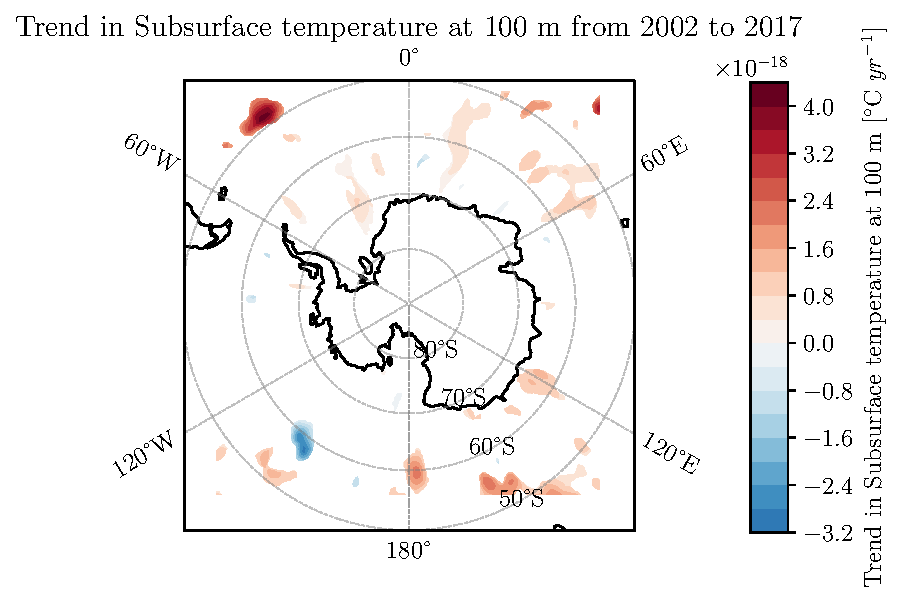
\includegraphics[width=\textwidth]{images/2021w5/chapter7/hres/trend_spatial_subsurtemp_100}
    \end{subfigure}
    \caption{Trend in subsurface oceanic temperature at different pressure levels over Antarctica from 2002 to 2017 \todo{make these sub-figures in python}. Only statistically significant trends have been plotted, i.e. with a p-value $\leq$ 0.05.}
    \label{fig:trend_subsurtemp_02_17}
\end{figure}

Looking at these sub-figures (figure \ref{fig:trend_subsurtemp_02_17}), we find like with \gls{skt} there are not many regions or a dominant pattern with a statistically significant trend in subsurface ocean temperatures at 100 dbar, 500 dbar or 700 dbar. 

We also want to consider the concentration of Ozone in the atmosphere at different levels. In literature this has been previously linked with land ice concentration change. \todo{cite this}. As such we consider the trend in ozone at different pressure levels. This data was sourced from the ERA5 reanalysis provided by ECMWF. We consider ozone mass mixing ratios at the same levels as other variables stratified \todo{check that I use stratified correctly} in the same manner, at 700 hPa, 500 hPa, and 200 hPa. We also want to consider what happens in the stratosphere as we know that ozone has been particularly dynamic there. So we also look at ozone mass mixing ratios at 100 hPa and 50 hPa. (See Figure \ref{fig:trend_o3_02_17}).

\begin{figure}[hbt!]
    \begin{subfigure}[b]{0.5\textwidth}
    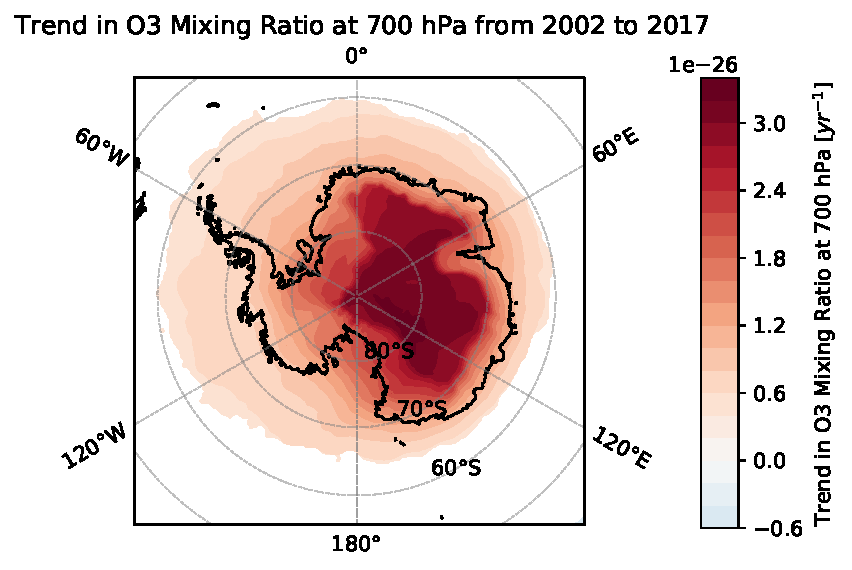
\includegraphics[width=\textwidth]{images/2021w5/chapter7/hres/trend_spatial_o3_700}
    \end{subfigure}
    \begin{subfigure}[b]{0.5\textwidth}
    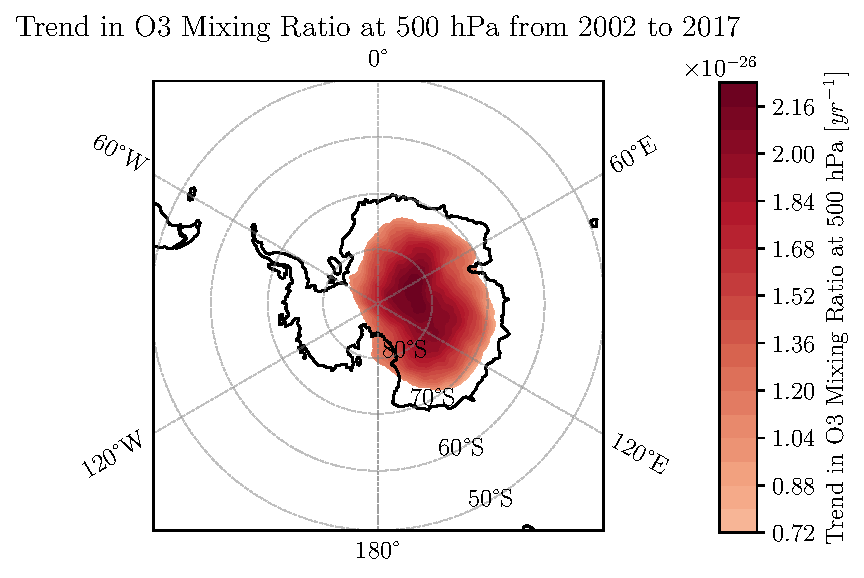
\includegraphics[width=\textwidth]{images/2021w5/chapter7/hres/trend_spatial_o3_500}
    \end{subfigure}
    \begin{subfigure}[b]{0.5\textwidth}
    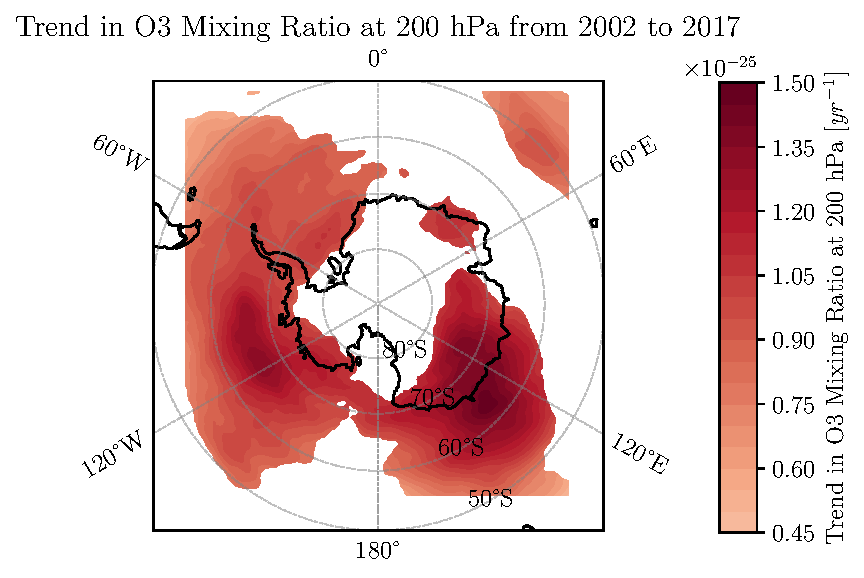
\includegraphics[width=\textwidth]{images/2021w5/chapter7/hres/trend_spatial_o3_200}
    \end{subfigure}
    \begin{subfigure}[b]{0.5\textwidth}
    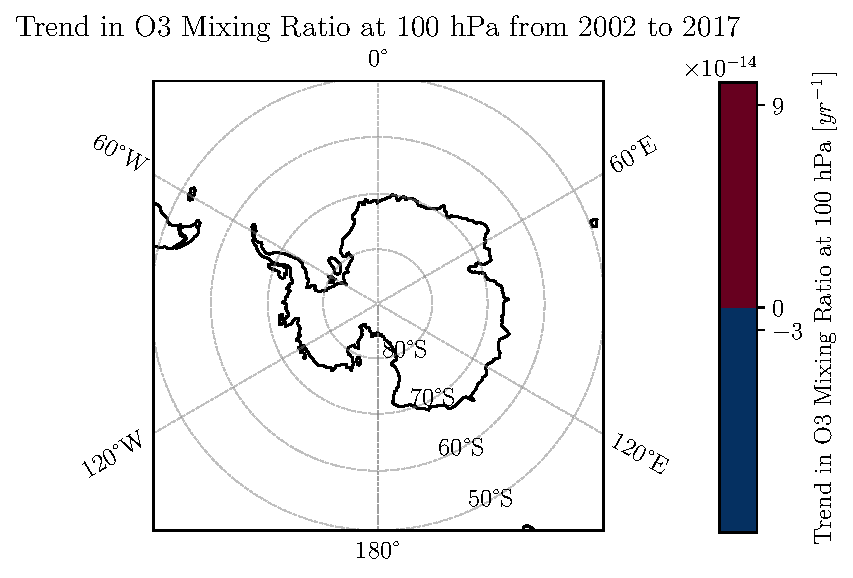
\includegraphics[width=\textwidth]{images/2021w5/chapter7/hres/trend_spatial_o3_100}
    \end{subfigure}
    \begin{subfigure}[b]{0.5\textwidth}
    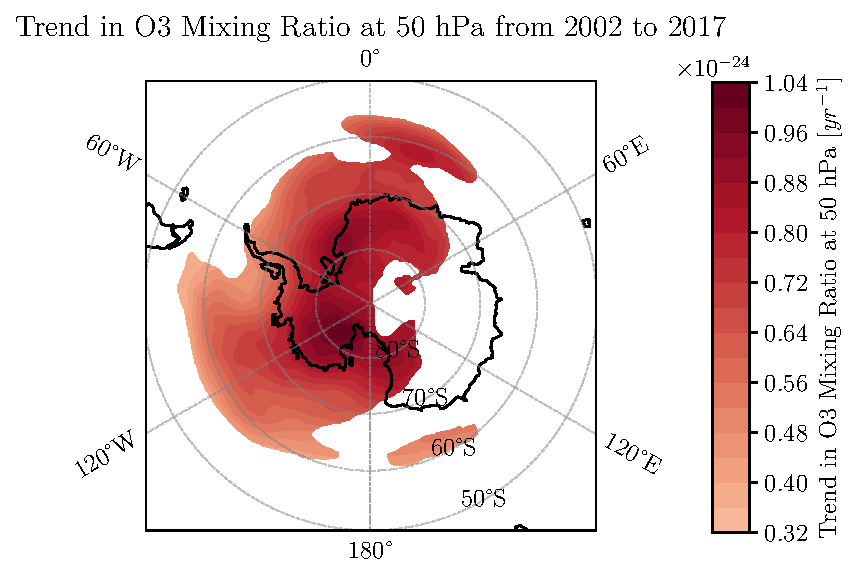
\includegraphics[width=\textwidth]{images/2021w5/chapter7/hres/trend_spatial_o3_50}
    \end{subfigure}
    \caption{Trend in ozone at different pressure levels over Antarctica from 2002 to 2017 \todo{make these sub-figures in python}. Only statistically significant trends have been plotted, i.e. with a p-value $\leq$ 0.05.}
    \label{fig:trend_o3_02_17}
\end{figure}

Looking at these plots we can make a couple observations. The ozone hole which has existed over Antarctica and has been disappearing over the last few decades.\todo{cite this} This is observed as a significant increase in ozone mass mixing ratio consistently over the entire continent at most pressure levels. We should note that no location has a significant trend for ozone at 100 hPa. At this level we do see some insignificant decreases in ozone.\todo{see if we know why this is the case or can find out quickly}

\missingfigure{Plot of trend wind speed}
\FloatBarrier
\section{Visual time series comparisons}
\todo{add plots for land ice and sea ice both}
Now we have some understanding of the spatial distribution of trends in each variable we also want to consider how they change over time and how that compares to the mean \gls{lilwet}. We do this by taking the average value for each variable over Antarctica. Only computing the average with locations where we have access to land ice data. We want to acknowledge before including these plots, that these plots represent a large region of spatial variability and as such should be used only as general indicators in the context of understanding the behaviour of the different variables. Nonetheless useful information can still be obtained here. We start by plotting the time series for mean \gls{skt} over land and mean \gls{lilwet} (see figure \ref{fig:timeseries_skt}).

\begin{figure}[hbt!]
    \centering
    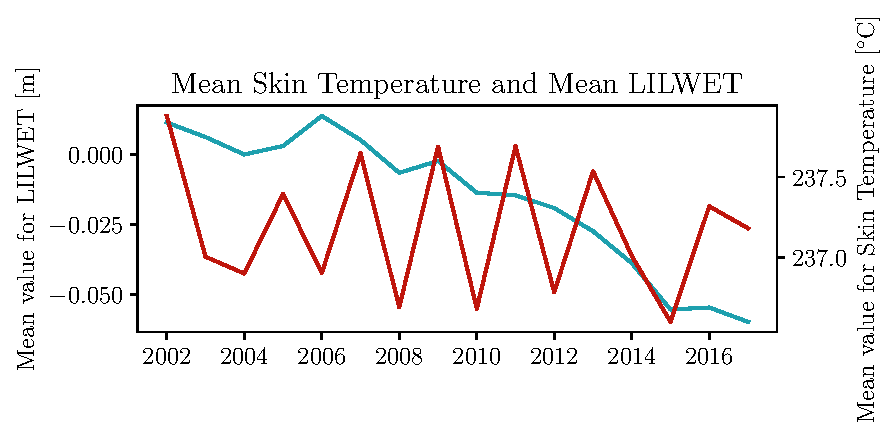
\includegraphics{images/2021w5/chapter7/hres/tiemseries_skt_LIC}
    \caption{Time-series of mean \gls{lilwet} and mean \gls{skt} over Antarctica. Mean is taken only over land.}
    \label{fig:timeseries_skt}
\end{figure}

Looking at Figure \ref{fig:timeseries_skt} we don't see many similarities between the two variables. We see a steady decrease in mean \gls{lilwet} and low variability. As opposed to skin temperature which exhibits high variability and a small trend \todo{say if increasing or decreasing trend} over the 16 years we are looking at. Given we found low correlations between these variables in chapter \ref{chap:temp_and_ice}, the apparent differences between the two time-series is not surprising. 

\begin{figure}[hbt!]
    \centering
    % 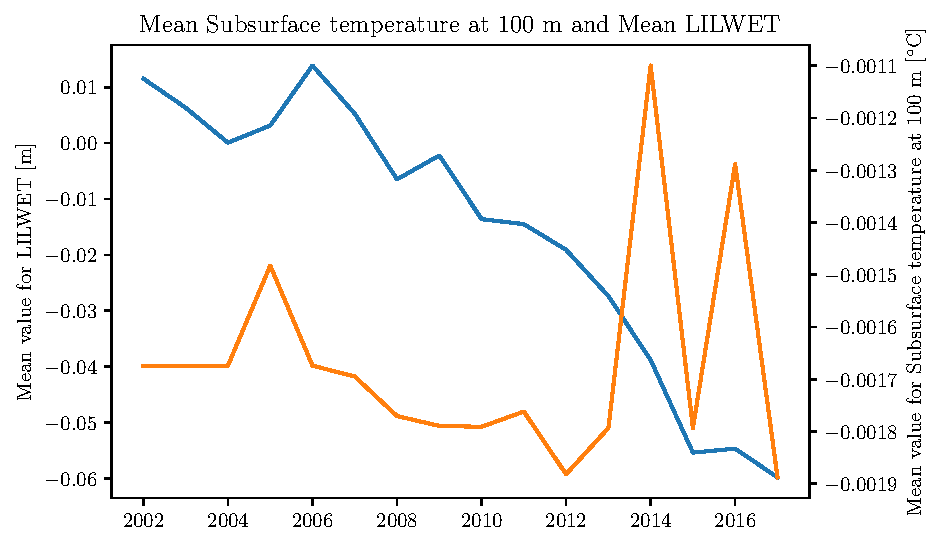
\includegraphics{images/2021w5/chapter7/hres/tiemseries_subsurtemp_100_LIC}
    \begin{subfigure}[b]{0.45\textwidth}
    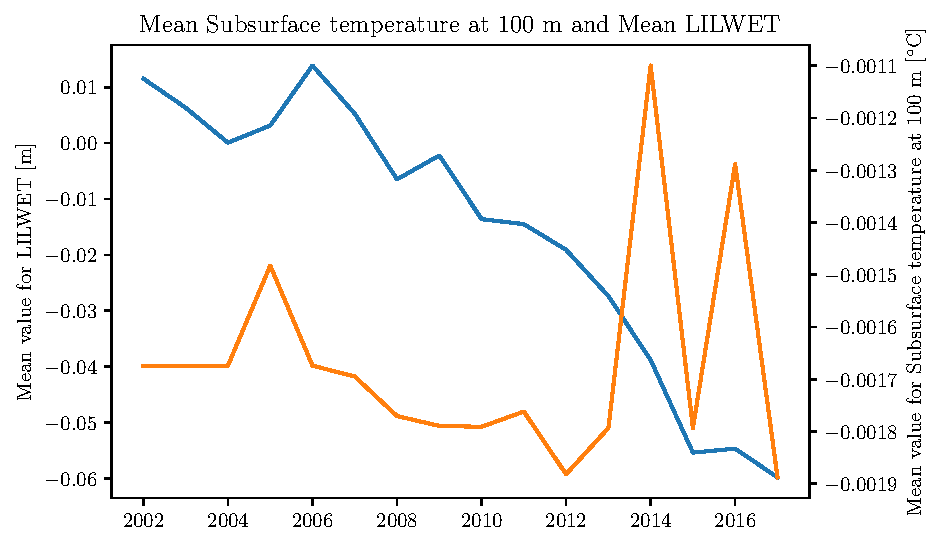
\includegraphics[width=\textwidth]{images/2021w5/chapter7/hres/tiemseries_subsurtemp_100_LIC}
    \end{subfigure}
    \begin{subfigure}[b]{0.45\textwidth}
    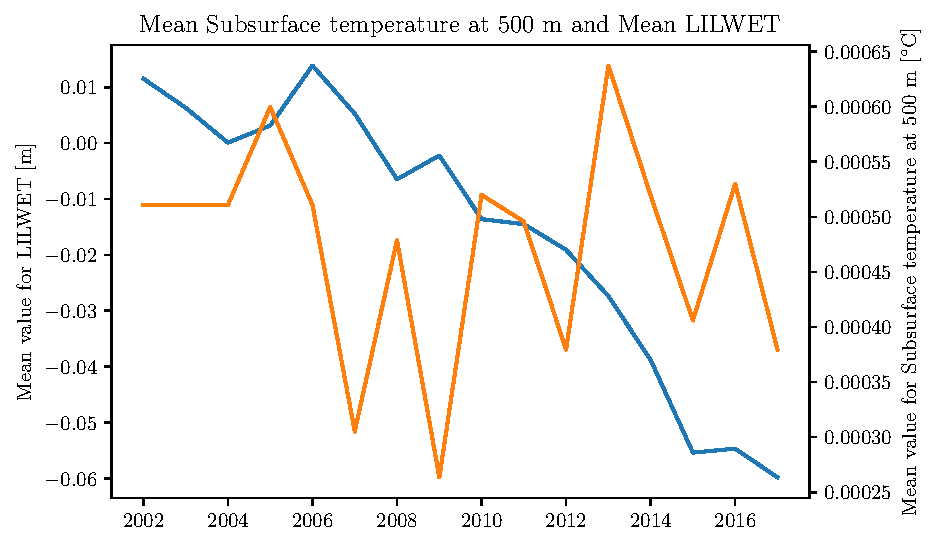
\includegraphics[width=\textwidth]{images/2021w5/chapter7/hres/tiemseries_subsurtemp_500_LIC}
    \end{subfigure}
    \begin{subfigure}[b]{0.45\textwidth}
    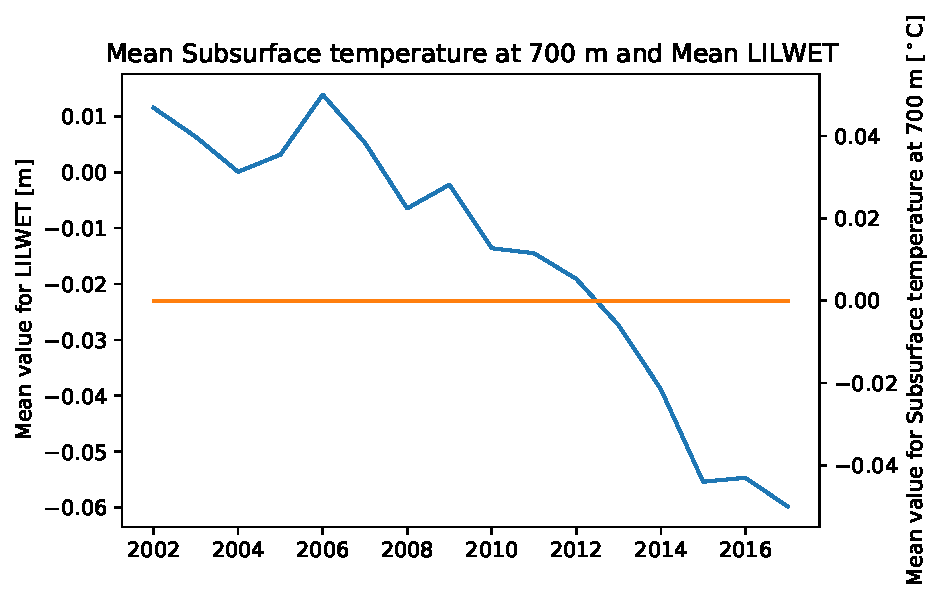
\includegraphics[width=\textwidth]{images/2021w5/chapter7/hres/tiemseries_subsurtemp_700_LIC}
    \end{subfigure}
    \caption{Time-series of mean \gls{lilwet} and mean subsurface temperature over Antarctica. As the variables do not coexist at the same location, no masking was applied to either variable.}
    \label{fig:timeseries_subsurtemp_100}
\end{figure}

Figure \ref{fig:timeseries_subsurtemp_100} is different to the other plots \todo{fix subsurface temperature timeseries plot}because the two variables do not coexist. So instead of taking only locations over land, we considered the mean subsurface temperature south of $55^\circ$S. \todo{write up anything interesting.}

\begin{figure}[hbt!]
    \centering
    % 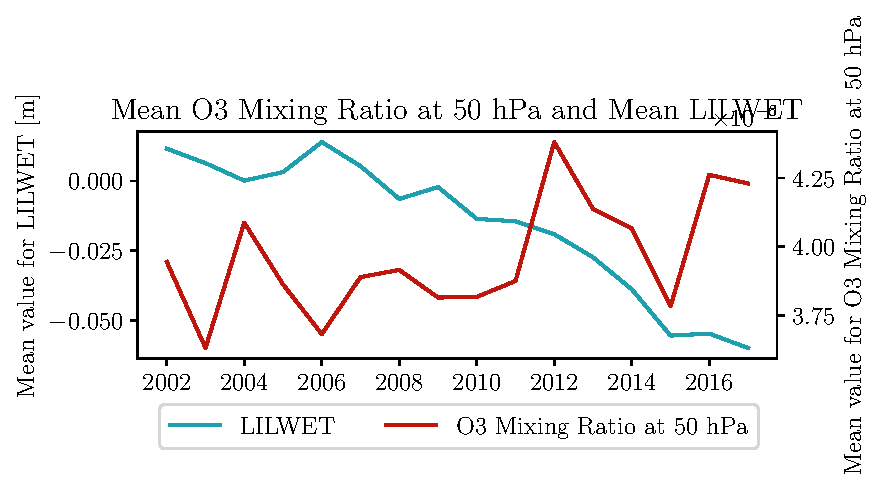
\includegraphics{images/2021w5/chapter7/hres/tiemseries_o3_50_LIC}
    % \begin{subfigure}[b]{0.45\textwidth}
    % % 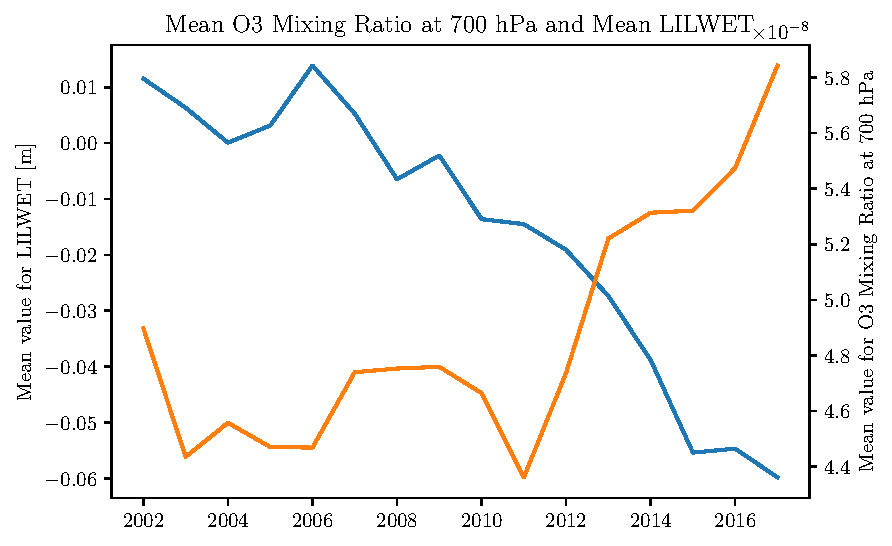
\includegraphics[width=\textwidth]{images/2021w5/chapter7/hres/tiemseries_o3_700_LIC}
    % 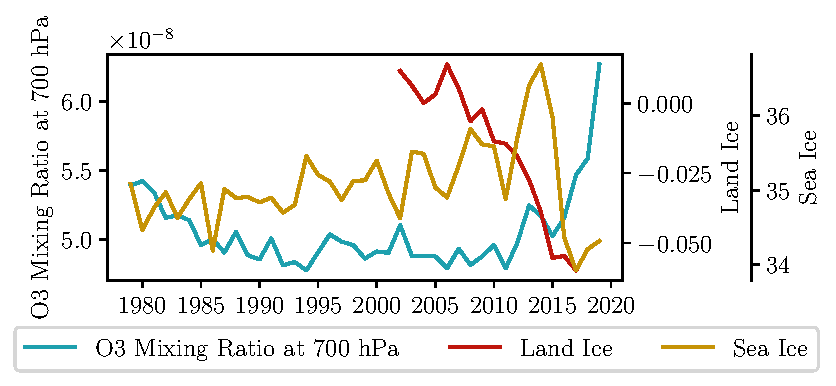
\includegraphics[width=\textwidth]{images/T2/timeseries_ice/hres/o3_700}
    % \end{subfigure}
    % \begin{subfigure}[b]{0.45\textwidth}
    % % 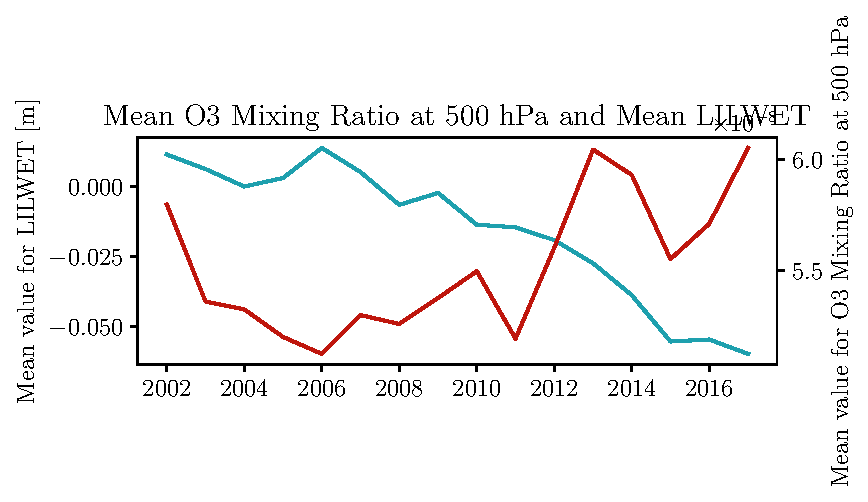
\includegraphics[width=\textwidth]{images/2021w5/chapter7/hres/tiemseries_o3_500_LIC}
    % 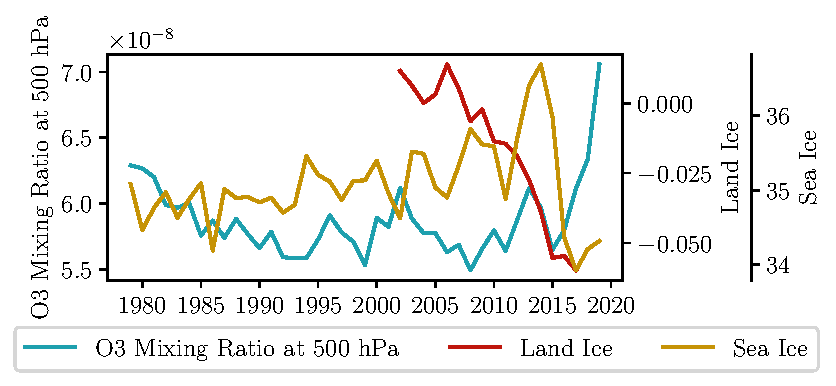
\includegraphics[width=\textwidth]{images/T2/timeseries_ice/hres/o3_500}
    % \end{subfigure}
    % \begin{subfigure}[b]{0.45\textwidth}
    % % 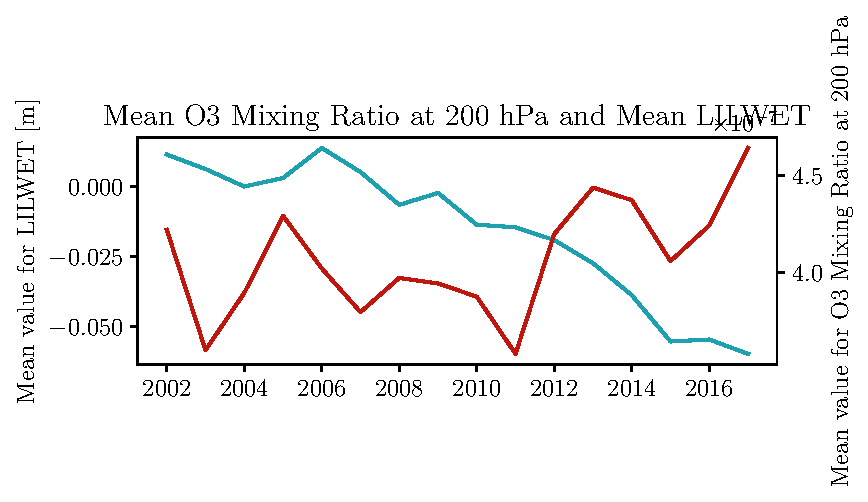
\includegraphics[width=\textwidth]{images/2021w5/chapter7/hres/tiemseries_o3_200_LIC}
    % 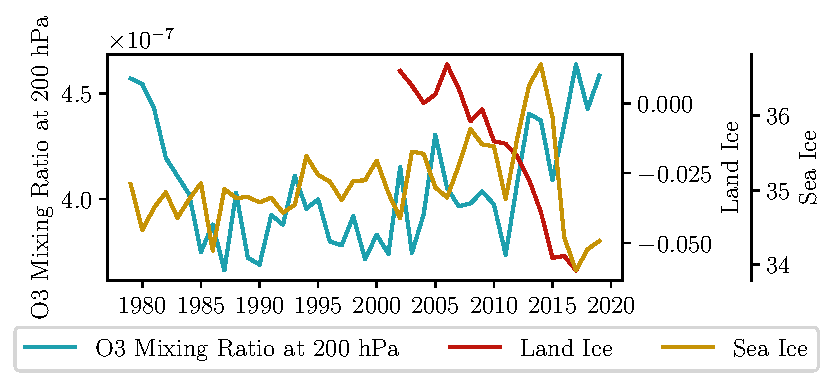
\includegraphics[width=\textwidth]{images/T2/timeseries_ice/hres/o3_200}
    % \end{subfigure}
    % \begin{subfigure}[b]{0.45\textwidth}
    % % 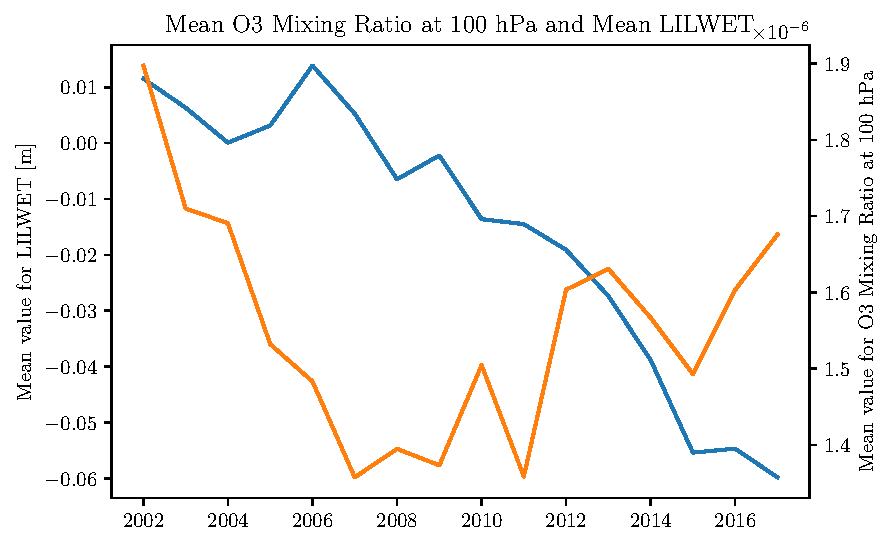
\includegraphics[width=\textwidth]{images/2021w5/chapter7/hres/tiemseries_o3_100_LIC}
    % 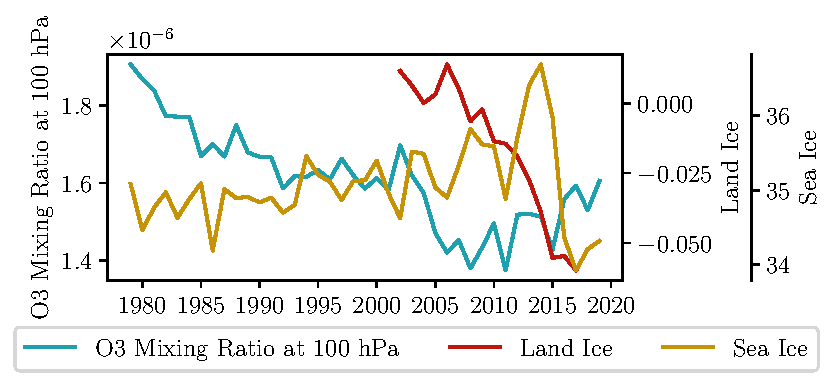
\includegraphics[width=\textwidth]{images/T2/timeseries_ice/hres/o3_100}
    % \end{subfigure}
    % \begin{subfigure}[b]{0.45\textwidth}
    % % 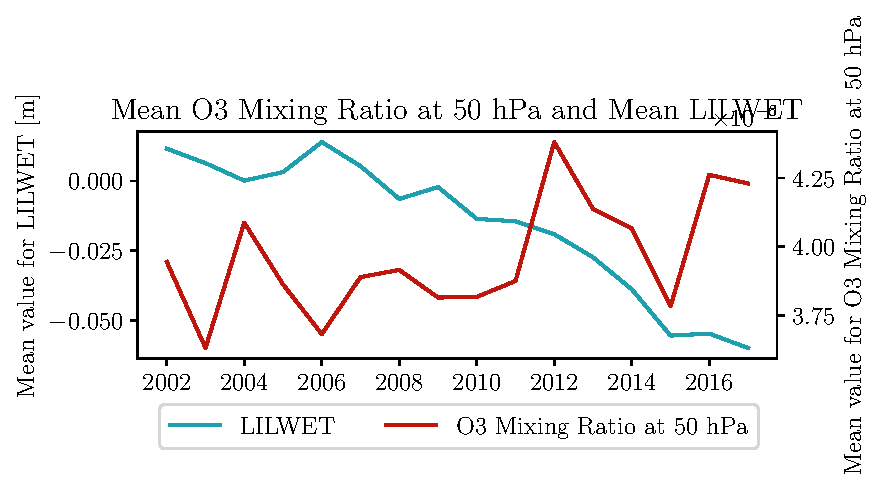
\includegraphics[width=\textwidth]{images/2021w5/chapter7/hres/tiemseries_o3_50_LIC}
    % 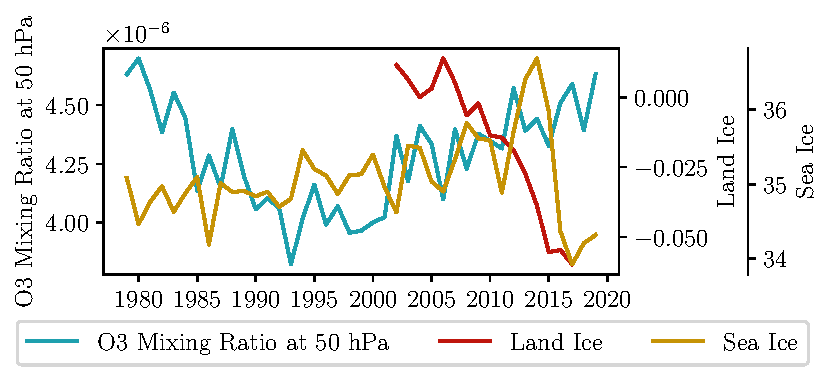
\includegraphics[width=\textwidth]{images/T2/timeseries_ice/hres/o3_50}
    % \end{subfigure}
    \includegraphics[width=\textwidth]{images/T2/subpl}
    \caption{Time-series of mean \gls{lilwet}, mean \gls{sic} and mean ozone mass mixing ratio over Antarctica at 50 hPa, 100 hPa 200 hPa, 500 hPa, and 700 hPa. Mean is taken only over land.}
    \label{fig:timeseries_o3_50}
\end{figure}

Figure \ref{fig:timeseries_o3_50} shows us the mean ozone mass mixing ratios at different pressure levels and the mean \gls{lilwet}.\todo{write this up once we have the figure.}

\begin{figure}[hbt!]
    \centering
    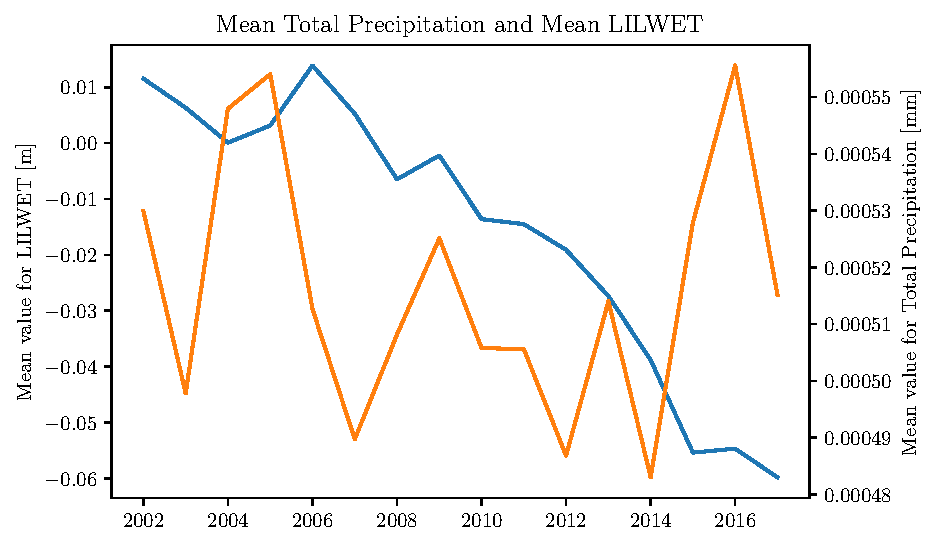
\includegraphics{images/2021w5/chapter7/hres/tiemseries_tp_LIC}
    \caption{Time-series of mean \gls{lilwet} and mean total precipitation over Antarctica. Mean is taken only over land.}
    \label{fig:timeseries_tp}
\end{figure}

We also looked at total precipitation. (see figure \ref{fig:timeseries_tp}) The idea being that changes in precipitation could be linked to changes in the amount of land ice as precipitation in the form of snow is a major mechanism for adding ice to the glaciers. Looking at the figure however we see no obvious similarity between the variables, so we will be cautious as we advance our analysis.

\begin{figure}[hbt!]
    \centering
    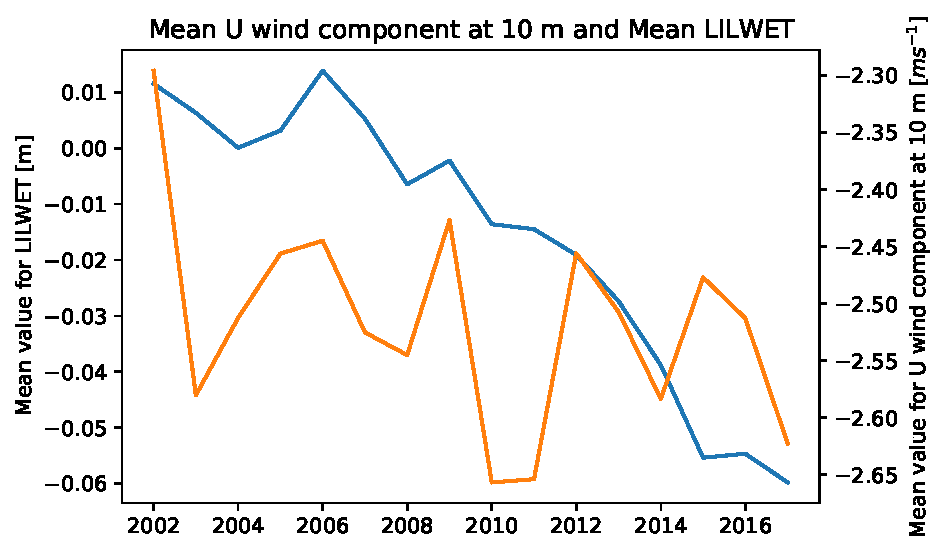
\includegraphics{images/2021w5/chapter7/hres/tiemseries_u_10_LIC}
    \caption{Time-series of mean \gls{lilwet} and mean wind speed over Antarctica. Mean is taken only over land.}
    \label{fig:timeseries_u_10}
\end{figure}\todo{do total wind speed for this plot at different levels}

We also looked at the behaviour of wind in relationship with \gls{lilwet}.\todo{finish writing up wind velocity time series.}

Looking at these plots, we do not have much to go off. Most of the variables show little to no similarity to \gls{lilwet}. As mentioned at the start of this section, this may be due to the information lost by taking the spatial mean of each variable across the entire continent. We will continue with our analysis by calculating the regressions of these variables with \gls{lilwet}, however with a grain of salt. 

\FloatBarrier

\section{Regression Analysis}

\begin{figure}[hbt!]
    \centering
    \begin{subfigure}[b]{\textwidth}
    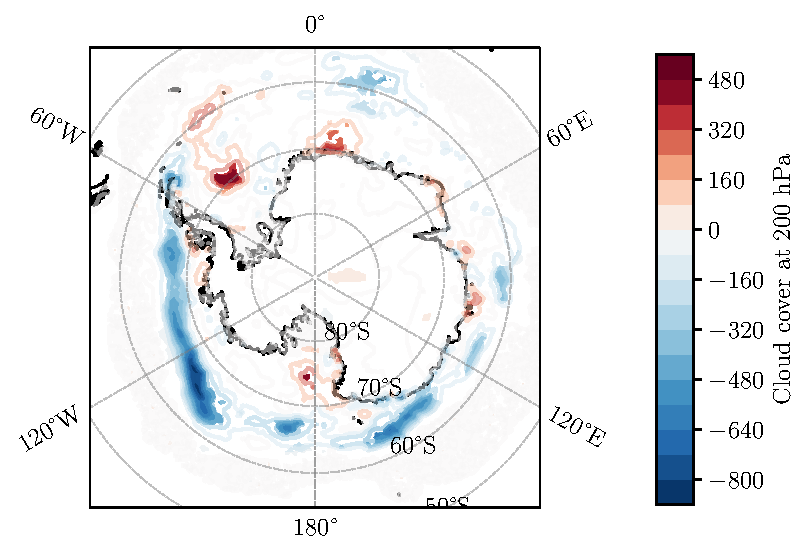
\includegraphics[width=\textwidth]{images/T2/single_regression/hres/cc_200_0.05}
    \end{subfigure}
    \begin{subfigure}[b]{\textwidth}
    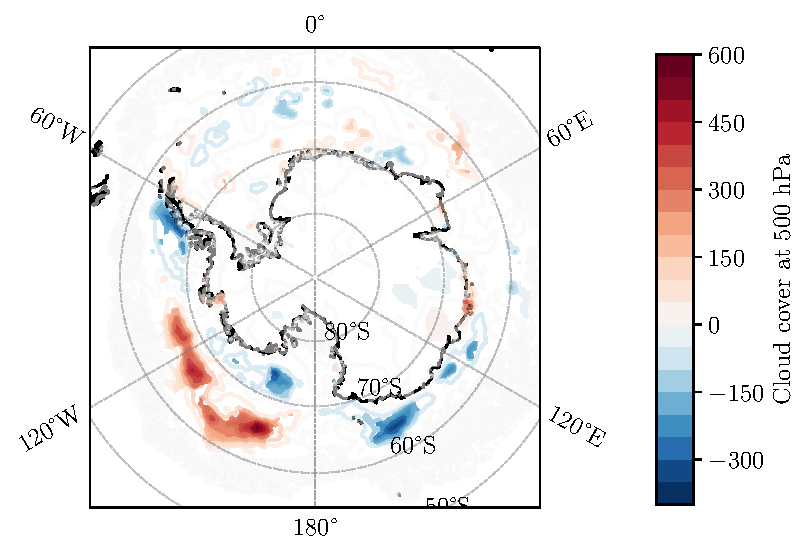
\includegraphics[width=\textwidth]{images/T2/single_regression/hres/cc_500_0.05}
    \end{subfigure}
    \begin{subfigure}[b]{\textwidth}
    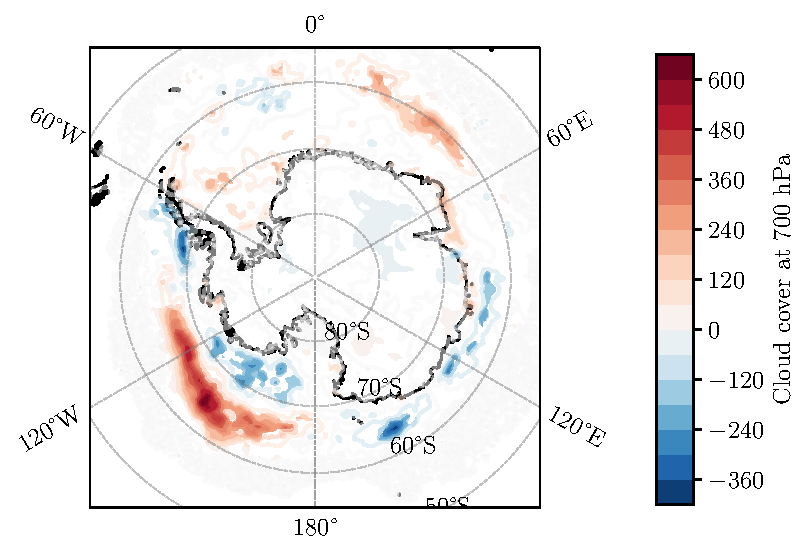
\includegraphics[width=\textwidth]{images/T2/single_regression/hres/cc_700_0.05}
    \end{subfigure}
    \caption{Regressions of cloud cover onto Antarctic Ice. Land ice and Sea ice regressions.}
    \label{fig:my_label}
\end{figure}

\section{Multiple Regression Analysis}





\end{document}